%-------------------------------------------------------------------------
% Design Project Input/Output Module Description
%-------------------------------------------------------------------------

\clearpage
\section{Flex Input Module}
\label{sec-input-flex}

This input module enables your IoT device to sense the flexing of a
\wu{6}{cm} strip. This may be useful in medical devices, physical
therapy, stress relief technology, virtual motion, computer peripherals,
etc. The flex sensor is a variable resistor whose resistance depends on
how much the strip is flexed (i.e., by bending it); the resistance is
higher when flexed in one direction and lower when flexed in the other.
The Arduino cannot directly sense resistance, but it can sense an analog
input voltage. We will use a simple circuit called a voltage divider so
that the voltage across the flex sensor is proportional to the
resistance.

A sample circuit and Arduino code is shown below to get you started.
The circuit places a \wu{10}{k$\Omega$} resistor in series with the flex
sensor so that voltage is divided between the two components. A
\wu{10}{k$\Omega$} resistor has brown-black-orange bands. We use a wire
to connect the node in between the resistor and the flex sensor to an
analog input of the Arduino so that the Arduino can read the voltage
from one end of the \wu{10}{k$\Omega$} resistor to ground. The example
code will print the analog reading from the flex sensor on the serial
monitor, similar to how we printed the analog reading from the grayscale
sensor in Lab~2. After setting up the circuit and programming the
Arduino, open the serial monitor and check what the sensor is reporting
regarding how much the strip is flexed. Try flexing the sensor strip in
one direction. Does the reading increase or decrease? Try flexing the
sensor strip in the other direction. Can you explain this behavior?

\vspace{0.1in}
\begin{minipage}[t]{0.49\tw}
  \vspace{0pt}

  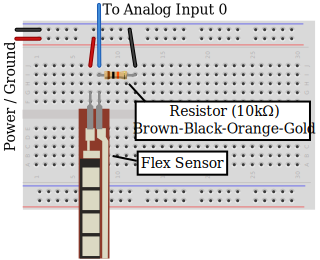
\includegraphics[width=\tw]{input-flex-annotated.svg.pdf}
\end{minipage}
\hfill
\begin{minipage}[t]{0.49\tw}
  \vspace{0.1in}
  \begin{Verbatim}[gobble=3,fontsize=\small]
    int pin_flex = A0;

    void setup() {
      Serial.begin(9600);
      pinMode( pin_flex, INPUT );
    }

    void loop() {
      int flex = analogRead( pin_flex );

      Serial.println( flex );
      delay(1000);
    }
  \end{Verbatim}
\end{minipage}
\vspace{0.1in}

%Questions:
